\section{XML Databases}

  XML is used as interchangeable data format in the web or for creating semi-structured documents such as XHTML. There is a necessity to store XML documents in a repository or database that helps for easy data storage and retrieval. An XML document can be stored in two different ways in a database. The first is to convert XML data into the database by mapping the document's data model to a database model. Databases that follow this method are called as \textit{XML-enabled databases}. The second is to find a persistent structure that can store any kind of XML documents and then XML model is mapped into it. Databases that follow this method are called as \textit{native XML databases} \cite{pavlovic2007native}. Though there is a choice to select any of these methods, it is more appropriate and efficient to store document-centric XML documents using native XML databases and data-centric  XML documents using XML-enabled databases. Native XML Databases (NXDs) are document-oriented databases, that store XML data and all the components of XML based on a logical model. The Logical model differs from individual NXDs where database must include at least an element, attributes, PCDATA\footnote{Parsed Character Data} and document order. This model includes different levels of complexity and complete support for mixed content and semi-structured data. NXDs can manage collection of documents, and also allow to query the documents. These databases are mainly suitable for storing irregular, recursive, and deeply hierarchical data.  BaseX, MarkLogic\footnote{http://www.marklogic.com/}, eXist-db\footnote{http://www.exist-db.org/}, Sedna\footnote{http://www.sedna.org/}, etc. are some of representative example of NXDs. 
  \par XQuery 1.0 and XQuery 3.0 are standard query languages recommended by W3C for NXDs. XQuery includes XPath as a sub-language for addressing specific part of an XML document. XPath is not really used as a querying language because it falls short in several ways such as grouping, sorting, support for data types and cross document joins. XSLT can be used to fill in these holes, and also to transfer XML to other documents like HTML, plain text and XSL Formatting Objects, but XQuery is more like a database oriented language.  The performance of queries in native XML databases can be improved using different types of indexes. Figure~\ref{fig:xml-indexes} shows the general indexing structure for an XML document. 
  In order to increase the performance of queries, NXD also has support for creation of indexes on the stored data\cite{pavlovic2007native}.
	\subsection{BaseX}
	BaseX is a native XML database management system and XQuery/XPath Processor that focuses more specifically in storing, querying and visualizing large XML documents. It uses tabular representation of XML data tree to store XML document~\citep{www/basex}. BaseX is a free software that facilitates the complete implementation of XQuery 3.0. To speed up the query evaluation process, BaseX has indexing mechanism. Due to complex tree structure of XML, there are wide range of index structures. Following are the most used types of indexes:
	\begin{description}
	\item[Name Index] \hfill \\
	It contains all element and attribute names of a database, and the ids are stored in the main table. The index is also provided with statistical information such as, minimal or maximum values of its elements and attributes. 
	
	\begin{comment}
	Name indexes and its contents can be directly accessed with XQuery functions \texttt{index:element-names} and \texttt{index:attribute-names}
	\end{comment}
	
	\item[Path Index] \hfill \\
	 It stores all the paths of documents in the database. In case of an database update, the statistics are discarded. With path index descendant steps can be rewritten into child steps, as child steps are evaluated faster.
	 \begin{comment}
	 and it can be created by \texttt{OPTIMIZE} command
	 \end{comment}
	 
	 \item{Text and Attribute Index] \hfill \\ This index increases the speed and range tests on text and attribute values. 
	 \begin{comment}
	 To keep the index up-to-date \texttt{UPDINDEX} option can be used. \texttt{index:attributes} can be used to access the index contents
\end{comment}
	  	 \item[Full-text Index] \hfill \\
	  	 In this indexing, there are two different types of indexes that are provided. One is the default index structure that sorts all keys alphabetically with respect to their character length. The second has a trie structure and takes more memory. 

\begin{comment} 
	  	 \texttt{contains-text} can be used to speed up full text indexing queries.
\end{comment}

\end{description}


\begin{figure}[h]
    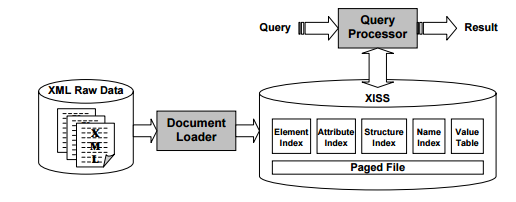
\includegraphics[width=1\textwidth]{img/Indexing}
    \label{fig:xml-indexes}
    \caption{Index in XML database~\cite{li2001indexing}}
\end{figure}

	\section{NoSQL Database}
	NoSQL databases (Not Only SQL) are distributed data management systems that store unstructured and semi-structured data. They are mainly known for its features like scalability, performance and availability~\citep{hecht2011nosql}.
	
	\textit{Scalability} is one of the key features of NoSQL database systems where data instances are large and stored separately in different nodes. These databases are designed to store from terabytes to petabytes of data by trading-off its capacity to handle ACID properties to high scalability over a large number of nodes\cite{abramova2013nosql}. 	
	%\textit{Availability} 
   \par  Data in NoSQL is stored in commodity hardware in many servers, therefore network failures are common during data operation. If one or more nodes are unable to deliver the request of a client,  other nodes in the system can complete the operation without any loss. Data is replicated throughout the different nodes for fault tolerance.%System allows eventual consistency among the replicas of same the piece of data~\cite{nosql/comparision}
 %All the NoSQL databases are schema-less and they are read in a way that is tolerant to the changes.  
    \par 
NoSQL databases can be categorized into four categories based on the data model and design:
	\begin{description}
		\item[Key/Value store] \hfill \\ 
		The data representation of key/value stores are based on attribute pair, the data model expressed as collection of $<$$key$,$value$$>$ tuples. The key is unique and value can be varied. Since the values are uninterrupted arrays, keys are used to retrieve the stored data. They have very simple data structure and are schema free. Key/value stores are mostly used for simple operations, which are dependent on key attributes. The query operation on data can be uniquely performed by a key. The data can not be accessed or modified without a key. Some examples of key/value stores are DynamoDB\footnote{}, Riak\footnote{http://basho.com/products/riak-kv/},and Redis\footnote{http://redis.io/}.
		\item[Document-oriented databases] \hfill \\ 
	These databases	are based on semi-structured data model and unique key stores a value that has a tree like structure called \textit{document}. Attributes are key/value pair in JSON or in JSON like data format where data can be accessed by using key or specific value~\citep{hecht2011nosql}. Every document contains a special identifier key. Unlike in key/value stores, the values are not opaque and  they can be used to query the document. Document stores are schema free, so new attribute values can be added to the existing documents at any time. These documents are very convenient in schema migration tasks and data integration.  MongoDB, Couchbase, RethinkDB, and CouchDB\footnote{http://couchdb.apache.org/} are some example of this system.
		\item [Column family databases] \hfill \\
		They are also known as wide-column databases that store data table as a section of a column and each of the column can have  its own index structure. A graphical representation of column-family is given in  Figure~\ref{fig:column-family-2}. Column databases are suitable for heavy write and optimized for writing data to a smaller subset of records. It offer less flexibility than key stores as column families have to be predefined. Because of the tabular format, the graphical representation is similar to relational databases. Column family stores are more suitable for applications dealing with large amounts of data stored in the cluster, as it can be efficiently partitioned.  Cassandra\footnote{http://cassandra.apache.org/}, BigTable\footnote{} and HBase\footnote{http://hbase.apache.org/} are categorized as wide column database.
		\item[Graph databases] \hfill \\
		Graph databases stores data as a  graph in the form of nodes and edges similar to a social network. These databases are efficient in handling heavily linked data. Data with many relationships are more suited for graph database as the operations like recursive joins can be replaced by efficient traversals. Neo4J\footnote{http://neo4j.com/} and OrientDB\footnote{http://orientdb.com/orientdb/} are two example of this database.

\end{description}
	
\begin{figure}[h]
	\centering
	\subfloat[column based database~\cite{wuoverview}]{
		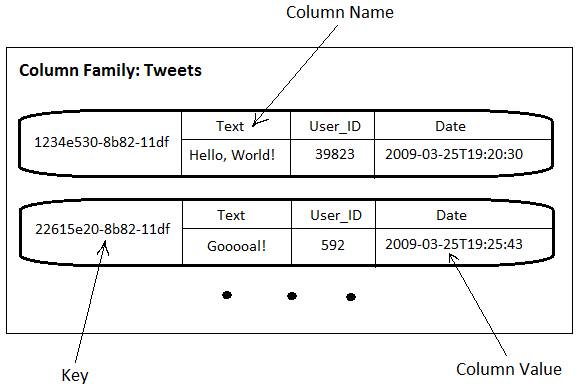
\includegraphics[width=.5\textwidth]{img/column-family}
		\label{fig:column-family-2}
	}
	\centering
	\subfloat[A document in document based database(JSON)]{
		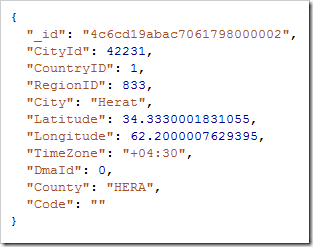
\includegraphics[width=.46\textwidth]{img/document-based-db}
		\label{fig:document-based-db}
	}
	\\
	\centering
	\subfloat[Graph database]{
		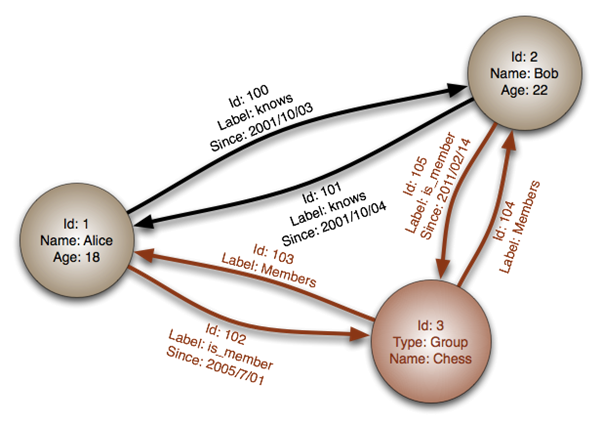
\includegraphics[width=.8\textwidth]{img/graph-database}
		\label{fig:graph-db}
	}
	\caption{column based database~\cite{wuoverview}}
	\label{fig:nosql-db-two}
	
\end{figure}

	\subsection{MongoDB}\label{nosql-mongodb}
	%MongoDB is schema-free database system that manage data in the concept of database, collection and documents. A database contains one or more collections(can be compare to tables of RDBMS) which stores documents. Collections may contain any type of documents but generally they have documents with  similar schema. Data has flexible schema where collections do not enforce document to structure rather requirements of the application. Documents are modeled as a data structure following the JSON format which actually store as BSON, a binary variant of JSON, supports additional data types like ObjectId, timestamp, datetime etc.
	MongoDB is a schema-less document-oriented database developed by MongoDB Inc. with the support of Open Source community. 
\subsubsection{Data design} 
\paragraph{Document}
	A document is abstract and storable unit in MongoDB. It is the data structure expressed in the form of JSON and is stored in BSON, a binary variant of JSON that supports additional data types like ObjectId, timestamp, datetime etc. All the accessible data including database records, query selectors, index specifications, server configurations etc. are represented as documents. An example  MongoDB document is given in Figure~\ref{sample-mongodb-document}.
Every document is referenced with a unique key. A document is retrieved either by the key or any other attribute of the document. Collection in MongoDB is a group of documents and it is stored in a database. It is more convenient to group similar structured documents in a collection but not mandatory. MongoDB has two principles that allow the users to represent the relationships between the documents: \textit{references} and \textit{embedded} documents~\citep{mongodb:org}. 
\begin{itemize}
\item {Embedded:}\label{mongo:embedded}
    In Embedded document, data is nested. The documents are structured as sub-document in the form of Arrays or Objects~\citep{nosql/comparision}. 
    \item{Reference:}
    Unlike RDBMS, MongoDB has no support for joins, therefore related data is stored in a single document. In some cases, the related data can be stored in a separate collection. The relationship between data can be created by including links and references from one document to another as shown in Figure~\ref{fig:mongodb-ref-doc}.  The references between the data can be created in two ways:
\begin{itemize}
	\item {\textbf{Manual references}}
		In manual references, the application handles the relationship between documents by referencing \textit{\_id} field of one document to other. 
	\item \textbf{Database reference}(\textit{DBRefs})
	In  DBRefs reference, a first document's primary index field, collection name and optional database name of a document is used to reference to another document.
\end{itemize}



	% 	A document can be refer to another document with the help of collections of references.  where as referencing both collection name and database, MongoDB allows a document reference to multiple database.   With the reference of collection, a document can be reference to another document belonging different collection.
\end{itemize}

\begin{figure}[h]
	\centering
	\subfloat[Reference document]{
		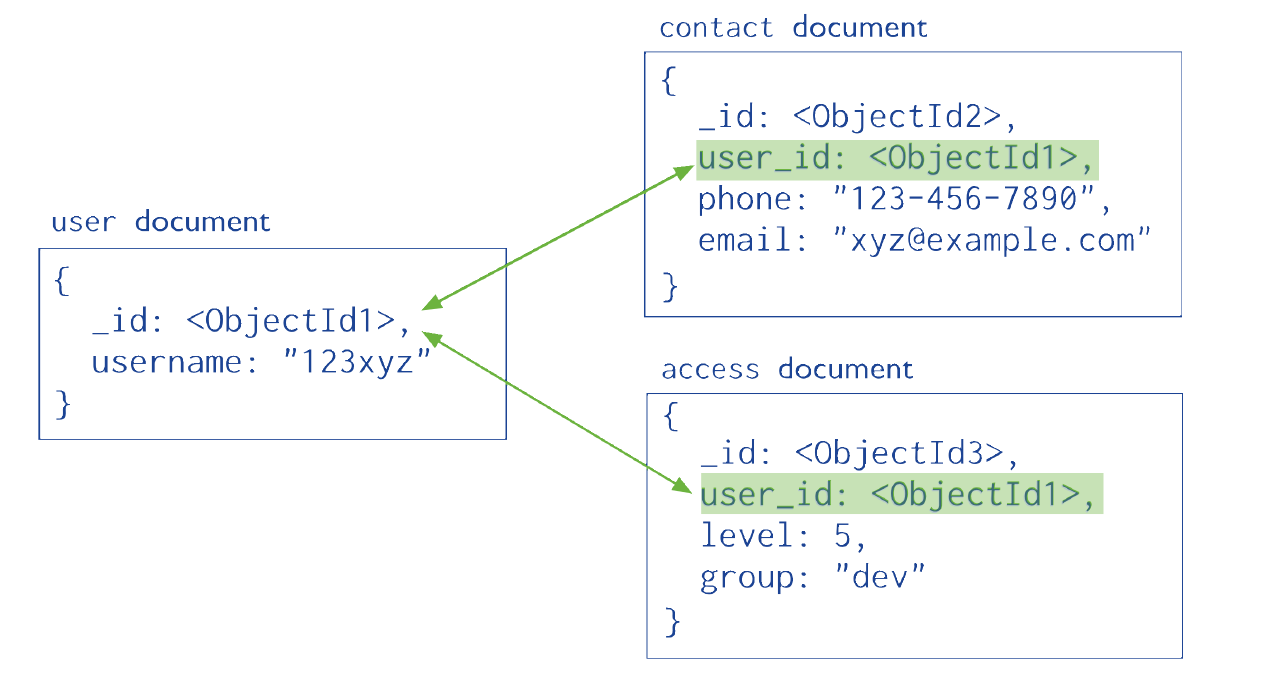
\includegraphics[width=.5\textwidth]{img/mongodb-reference}
		%{img/mongo/mongodb-reference}
		%\caption{R-tree structure}
		\label{fig:mongodb-ref-doc}
	}
	\centering
	\subfloat[Embedded document]{
		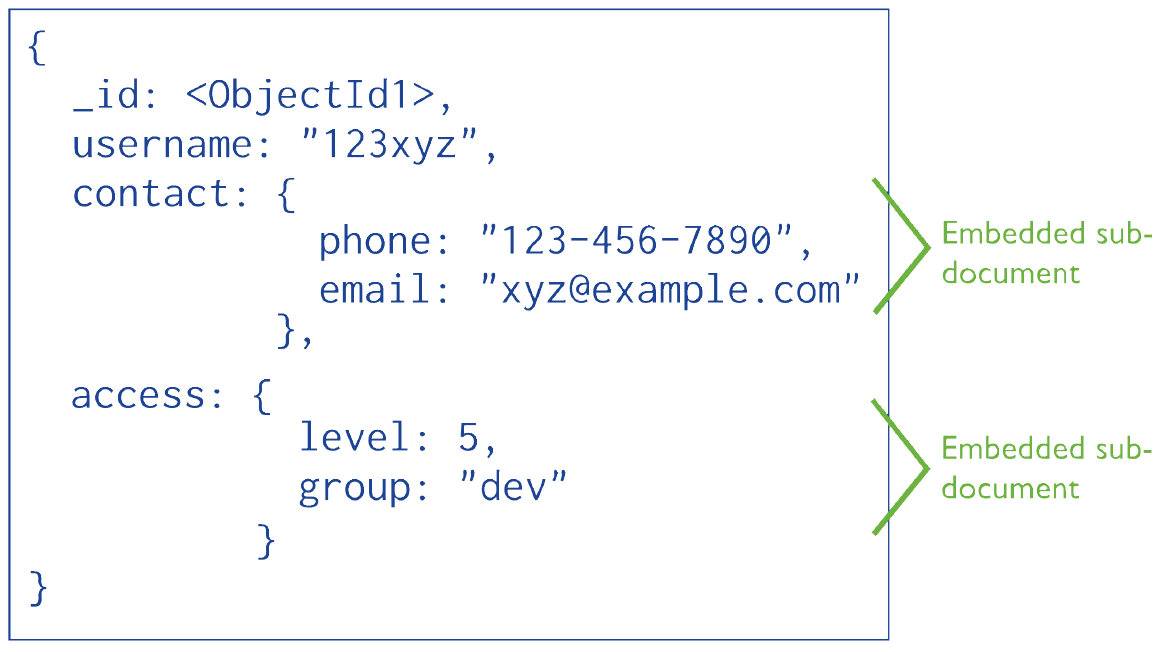
\includegraphics[width=.46\textwidth]{img/mongo/mongodb-embedded}
		%\caption{R-tree}
		\label{fig:mongodb-emb-doc}
	}
	\caption{MongoDB document structure~\citep{mongodb:org}}
	\label{fig:mongodb-doc}
	
\end{figure}

	\begin{figure}[h]
	\begin{lstlisting}[language=JSON,basicstyle=\scriptsize]
	{
		_id : "1"
		title : " MongoDB ",
		last_editor : "172.5.123.91" ,
		last_modified : new Date ("9/01/2015") ,
		body : " MongoDB is a..." ,
		categories : ["A", "B"] ,
		reviewed : false
	}
	\end{lstlisting} 
	\caption{MongoDB sample document}
	\label{sample-mongodb-document}
\end{figure}

\subsubsection{Indexing}\label{mong-xmark-indexing}

Each document in MongoDB is uniquely identified by a field \textit{\_id} which is also a primary index. Hence, the collection is sorted by \textit{\_id}~\citep{nosql/comparision}.
Apart from the primary index, MongoDB provides a mechanism to create secondary indexes for all fields of document. It supports various user defined indexes for field values including single field index, multikey index, multidimensional index, geo-spatial index, text index and hash index.
%Single field, multidimensional and multikey indexes are organized using B-tree, whereas geospatial index is implemented using quad trees.Once index is defined on a field,
\begin{itemize}
\item \textit{Single field index} only includes data from a single field of documents in a collection. 
\item \textit{Compound index} holds reference to the multiple fields within a collection's documents.
\item To index a field that contains an array value, MongoDB provides special indexing called \textit{Multikey index}.
\item \textit{Text index} helps efficient search of a string in documents.
\end{itemize}
\subsubsection{Query Model}\label{mongo-query-model}

%\todo{modify with christian's suggestions}
Queries in MongoDB are expressed in a JSON-like syntax and are sent to MongoDB as BSON objects by a database driver\citep{orend2010analysis}. A query can be specified by exact match on the embedded document or by using individual field with a \textit{dot notation}. It is used to access an element in document of an array or an object in the form of  $<$$array$.$index$$>$ or  $<$$object$.$childobject$$>$. For general queries, mongo shell can be used. It is an user friendly JavaScript shell that allows to implement callback functions to manipulate the data returned by the queries.  
\par
The Query model supports the following features:
\begin{enumerate}
	\item Queries over documents, embedded subdocuments and arrays
	\item Comparison operators
	\item Conditional Operators
	\item Logical Operators: AND and OR
	\item Sorting 
	\item Grouping
	\item Aggregation per query
\end{enumerate}

The \textit{find()} method is the most common way to retrieve data from a collection. It returns the subset of documents from specified collection with given criteria that are passed as parameters. If no any parameters is given, it returns everything from a collection.  The General syntax of find operation is given in Code~\ref{mongodb-find-sample}.
\begin{lstlisting}[language=JSON,caption=\textit{find} in MongoDB, label=mongodb-find-sample][H]
    db.collection.find(query, projection) 
\end{lstlisting}
 The \textit{query} specifies the criteria of document of a collection name \textit{collection}. The \textit{projection} selects of attributes of an documents to be return. For example, Code~\ref{mongodb-find-real} return the \textit{name} and \textit{age} from a collection  \textit{people} of country \textit{France} and \textit{age} is less than 5. 
\begin{lstlisting}[language=JSON,caption=\textit{find()} with query and project, label=mongodb-find-real][H]
    db.people.find({country:"France", age:{$lt:5}}, {_id:0, age:1, name:1}) 

\end{lstlisting}

\par
\paragraph{Aggregation Frameworks:}
 The \textit{find} method is not sufficient for the complex database queries like aggregation, grouping  and advanced data manipulation. MongoDB provides two frameworks for advanced query as well as parallel processing for the large collection:
 \begin{itemize}
		\item{ \textbf{Aggregation pipeline}} allows to execute series of operations using different operators like filtration, projection to produces desire result or performs aggregate operation.  It can be used for a single collection and uses  data operators like match, group, project, etc. in different stages. Every stage convert the documents as they pass through the pipeline. Data operators can be used  in any numbers of times.  The \textit{aggregate} function is responsible for this framework where it operates on a collection passing  entire documents into a pipeline. By using proper filtration operators like  skip, match and limit at the beginning  stage of the pipeline,  the frameworks can take advantages of existing indexes with processing scope limited to subset of documents, hence produces better performance in following stages~\cite{mongodbaggregation}. The aggregation pipeline has many limitations including data types, memory restriction to operators and output size~\cite{nosql/comparision}. Only 100 MB of RAM is assigned to pipeline stages. If this limit exceeds, the query will be broken. An option \textit{allowDiskUse} must be enable to write data to temporary files during staging.
		
				   \begin{lstlisting}[language=JSON,caption=An example Aggregation pipeline in MongoDB, label=mongodb-aggregation-pipeline, basicstyle = \scriptsize][h]
            db.open_auctions.aggregate([
                {$match:{reserve:{$exists:true}}},
		       {$project:{_id:0,reserve:{$multiply:["$reserve",2.20371]}}}
		       ]);
		  \end{lstlisting}
		  
		  \item{\textbf{MapReduce}} is a data processing framework design to support large volumes of data that goes beyond the limitations and restriction of aggregation pipeline.  In mapreduce,  \textit{map} function applies to each input document and emits the key-value pair as output. Any arbitrary sorting and limiting  of single collection is performed before map stage. The reduce applies to the map's output where a key is associated with multiple values to return the aggregated data. The output of \textit{reduce} may pass optionally through finalize function to further process the result. Mapreduce functions are written in JavaScript and executed in MongoDB's demon process ~\cite{mongodbaggregation}.  Unlike pipeline framework, Map-reduce support options for choosing to store result  data in a node as collection or return the output. Table~\ref{mongdb-mapreduce} illustrates a Mapreduce implementation in MongoDB. Two JavaScript function are defined for map and reduce. The \textit{runCommand} executes these functions in a collection.
		  
\end{itemize}		

\begin{longtable}{c|c}
\caption{Mapreduce in MongoDB}
 \label{mongdb-mapreduce}\\
	
	{\textit{map}} function(a) & {\textit{reduce}} function(b)\\
	\hline
	\begin{minipage}{.4\textwidth}
		\centering		
		\begin{lstlisting}[language=XML,basicstyle = \scriptsize,label=couchbase-map-sample]
map = function() {
           if(this.reserve){
            emit(this._id, this.reserve);
           }    
        };	
		\end{lstlisting}		
	\end{minipage} &
	\begin{minipage}{.49\textwidth}
		\centering
		\begin{lstlisting}[language=JSON, basicstyle =\scriptsize, label=couchbase-reduce-sample]
reduce = function(key,values) {
            return Array.sum(values);
        };
};
		\end{lstlisting}
	\end{minipage}
	\\
	\hline
	\multicolumn{2}{c}{
	    \scriptsize
	    
	Use: 	db.runCommand({"mapreduce" : 
	\textit{collectionName}, 
	                       "map" : \textit{map}, 
	                       "reduce" : \textit{reduce}})
		
	}
  	
  	\\
	\hline
	
\end{longtable}

%end here



\begin{comment}


\paragraph{System Architecture}
MongoDB can be run in two modes. In stand-alone mode, a single \textit{mongod} demon runs in a single node without any distribution and in shared mode various services are distributed to several nodes. 
\begin{figure}[h]
	\centering
	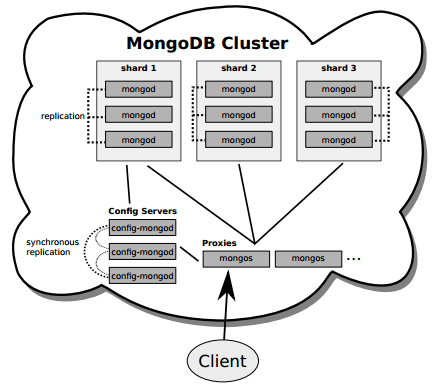
\includegraphics[width=0.5\textwidth]{img/mongo/clusters}
	%\caption{R-tree}
	\label{fig:mongodb-clusters}
\caption{MongoDB Clusters}
\end{figure} %reference




\end{comment}
	\subsection{Couchbase Server}\label{intro-couchbase}
	%Couchbase Server is NoSQL database that can be used both as a key-value store as well as document store system. As key-value store, it is able to store  multiple data type such as strings, numbers, datetime, and booleans as well as arbitrary binary data. The key-value generally treated as opaque Binary Large Object(BLOB) and don't try to parse it. For document store, data need to be store in the valid JSON format. Data in Couhbase Server are stored in logical unit called Buckets. These buckets can be technically compare as \texttt{database} in Mongodb or other RDBMS. All data type other than JSON can be retrieve only by their key. So it is important to check meta type of data stored in a single document before retrieval. Unlike MongoDB, Couchbase server Don't have concept of collections, so category of documents are identified by user defined type or group.
	 Couchbase Server is designed to be an operational data store for real-time data access. It is a NoSQL database that serves both as key-value and  document-oriented database. As a key-value store, it is able to store any type of data including  strings, numbers and binary data and the data is generally treated as an opaque Binary Large Object(BLOB) that do not try to parse it at the time of query. when being used as document store, data is stored in a valid JSON format. The data in Couchbase is stored in logical unit called buckets. These buckets  are isolated to each other and have their own RAM quota and replica settings. Buckets can be compared with \texttt{database} in Mongodb or other RDBMS. Couchbase recommends few numbers of buckets in a single cluster. A Bucket contains any type of data but data other than JSON, it can be retrieved only by its key. Therefore, it is important to check meta type of data that is stored in a single document before fetching. Each document is stored independently and there is not the notion of grouping documents like collections in MongoDB or tables in other RDBMS. The documents is separated by a user-defined type to distinguish the such documents.  For example, all the documents that are in \textit{user} and \textit{post} collections of MongoDB can be represented in Couchbase by adding a new field \textit{documentType}  in each document  with value \textit{user} and \textit{post} respectively.  
\label{cb-metadata}
\paragraph{Metadata}
For every value stored in a bucket, Couchbase Server generates following meta information that is associated with a document~\cite[p. 26]{cb/ostrovsky2014pro}. 
\begin{itemize}
	\item{Expiration}
		The Time to Live(TTL) also named as expiration time is the life time of the document. The default value of TTL is 0 that indicates document will never expire and also can be set as Unix epoch time after which document is removed.
	
	\item{Check-and-Set(CAS)}
		The CAS value is 64-bit integer that is updated by server when associated item is modified. It enables to update information only if unique identifier matches the identifier of the document that needed to be updated. CAS is used to manage concurrency when multiple client attempts to update the same document simultaneously. 
	\item{Flags} are 32 bit integer and are set of SDK specific use. For example, format in which data is serialize or data type of the object being stored.
\end{itemize}	
In addition of TTL, CAS and flags, three other meta information are stored at the time of document creation. The document's key \textit{id} is saved as part of metadata, \textit{type} is the type of a document either \textit{json} or Base64 encoded string for all other.
\paragraph{\textit{Document key}}
Every value in Couchbase Server is saved in unique key called document key. Unlike MongoDB, Couchbase  do not generate document key automatically and 250 characters string should be manually generated.
%In case of XMark data each \texttt{id} attributes of  \texttt{item}, \texttt{person}, \texttt{open\_auction}, \texttt{category} represent as key. In case of  \texttt{closed\_auction} and  \texttt{edge} key can be manually generated. 
\begin{figure}[h]
	\centering
	\subfloat[Views in Document Design]{
		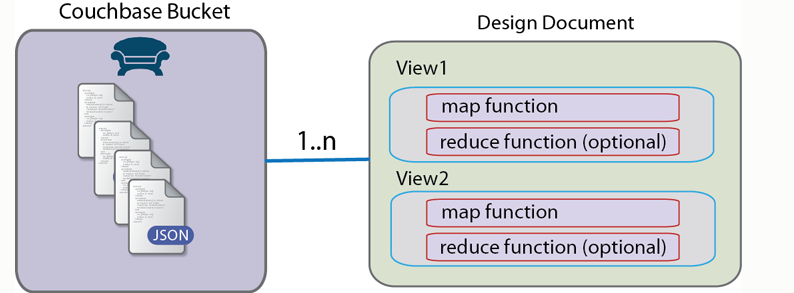
\includegraphics[width=0.4\textwidth]{img/cb/Small_view_elements}
		\label{fig:cb-views-design}
	}
	\centering
	\subfloat[View's Workflow]{
		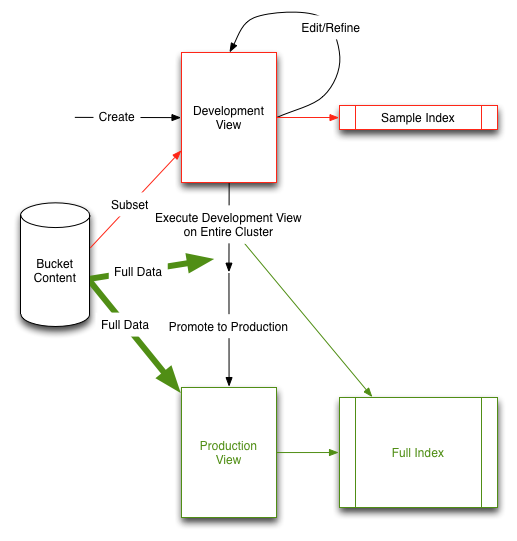
\includegraphics[width=0.4\textwidth]{img/cb/view-types-workflow}
		\label{fig:cb-views-workflow}
	}
	\caption{Couchbase Server's Document Design ~\citep{couchbasedocs}}
	\label{fig:cb-views-document-design}	
\end{figure}

\paragraph{Bucket and vBucket}
Couchbase Server uses data bucket as a logical container of information that provides a logical grouping of physical resources within a cluster~\citep{lichtenberg2013nosql}. Documents in Couchbase do not have their fixed schema and multiple documents  with different schema can be stored in same bucket. One or more attributes in documents are added to differentiate the various objects stored in a bucket and create indexes on them. Each bucket is split into 1024 logical partition called vBuckets. A vBucket is treated as a owner of subset of key where every key belongs to a vBucket~\ref{fig:cb-vbucket}.  
%%why we need vbucket

\begin{figure}[h]
	\centering
	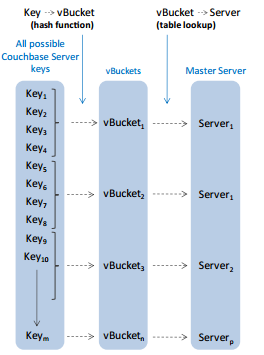
\includegraphics[width=0.4\textwidth]{img/vbucket2}
	\caption{ Couchbase  vBucket ~\cite{couchbasedocs}}
	\label{fig:cb-vbucket}
\end{figure}
%where is reference of images

\paragraph{Data Model}%repeat check once
A document is a basic unit of data manipulation in Couchbase  as a document store. All the documents are stored in JSON format without a predefined schema.

\paragraph{Querying and Indexing}
Query in Couchbase has to be done against pre-materialize views. The goal of view is to select the data, extract the attributes and information as client's need  and to produce the index on selected information. Views are defined in a specific kind of document called \textit{design document}~\ref{fig:cb-views-design}. These documents are bounded to a single bucket and cannot be executed from other bucket. The design document holds JavaScript code that implements \textit{Mapreduce} operations to create view's index in user defined format. The Mapreduce is achieved by two functions \textit{map} and reduce. Table~\ref{tbl:cb-mapreduce} illustrate a sample mapreduce function in Couchbase.

The \textit{map} function in design document identifies data from collection, process, filter them and output transformed values. Each document in a bucket is submitted to the \textit{map } function where document and metadata associated with the document are supplied as parameter to the \textit{map} function. After filtration, the \textit{emit} function in map returns the result as set of key/value pairs that are index. The output of map function can be zero or more "rows" according to the filter used in \textit{emit()} function. Each \textit{emit()} function returns a single row but can be called multiple times inside a single map function. The first parameter in \textit{emit} function is searchable text key and second parameter is the value.
The \textit{reduce} function is used to aggregate the numeric value generated in map phase. Couchbase has built-in reduce functions like \textit{\_count}, \textit{\_sum} and \textit{\_stats} aggregation. Table ~\ref{tbl:cb-mapreduce} illustrate an example of MapReduce  in Couchbase. The emit function at map phase returns the \textit{id} of document  as key and the price greater than 40 from documents that contains \textit{doctype} value "closed\_auctions". In \textit{reduce} phase, the the keys are grouped and values are counted.

%start here 
 In contrast to MongoDB,  Couchbase's queries are closely associated with client SDK where each operations has to perform through SDKs. On-demand query language  named "N1QL" is also in  progress of development but still stable version has to be released~\cite{couchbasen1ql}.


%end here from benchmarking sections.
\begin{table}[H]
\begin{longtable}{c|c}
	\caption{Mapreduce in Couchbase}
	\label{tbl:cb-mapreduce}\\
	\textit{map()} & \textit{reduce()}\\
	\hline
\begin{minipage}{.6\textwidth}
\begin{fakeJSON}[label=cb-mapreduce-map,basicstyle =\scriptsize]
function (doc, meta) {
   if(doc.doctype && doc.doctype=="closed_auctions"){
     if(doc.price){
       if(doc.price > 40) {
	      emit(doc.id,doc.price)
     	}
    }
  }
}

\end{fakeJSON}	
\end{minipage} &
\begin{minipage}{.2\textwidth}
\begin{fakeJSON}[label=cb-mapreduce-reduce]
	_count
\end{fakeJSON}
\end{minipage}\\
\end{longtable}
\end{table}


	
	\subsection{RethinkDB}
	%RethinkDB is distributed database system to store  JSON documents that uses efficient query languages named ReQL which automatically parallelize queries in multiple machines. RethinkDB has similar concept of store database like MongoDB. A database contains schema-less table, where documents are stored in the form of JSON. Unlike MongoDB, RethinkDB query language supports join queries between tables.
	RethinkDB is an open-source distributed document-oriented database system to store JSON documents. One of the unique feature of RethinkDB is the changefeed by the server to the client. 
Instead of a client request, the changes in database is streamed to the client application in realtime. In case of multi-users environment, any database  update is automatically notified.
\par
ReQL is the query language  of RethinkDB and it is based on three main principles:
 \begin{itemize}
 \item  It is  embedded  as programming language. Queries are constructed by making function call. 
 \item ReQL queries are chainable that can be passed as pipeline from one stage to another. Complex operation can be performed using series of simple queries together by using dot operators (\.) . 
 \item All the queries are executed in server without any intermediate network round trip between the server and clients.
 \end{itemize}
  
\subsubsection{Data Model}
There are two ways to model relationships between the documents: 
\begin{itemize}
	\item \textbf{Embedded arrays:} In this method, the related sub-documents are inserted with a specific key inside a document as in MongoDB ~\ref{mongo:embedded}. The advantages of using embedded arrays are:
		\begin{itemize}
			\item The Queries tend to be simpler. 
			\item If a dataset  does not fit into RAM, then the data is loaded  from the disk and it is faster compared to tables. 
		\end{itemize}
		Disadvantages of embedded arrays are: 
		\begin{itemize}
			\item Before any operation, data should be loaded into memory. In case of any updates, the document will rewrite the full array to the disk.
		\end{itemize}
		
	\item 
	\textbf{Multiple Table Approach:} In this approach, documents with similar structures are stored in multiple tables similar to collection in MongoDB. These tables are connected by reference key. Unlike embedded arrays, operation of a table does not required to load data from reference table in memory.
\end{itemize}

\subsubsection{Query Model}
RethinkDB's query language ReQL is embedded as programming language and JavaScript expressions can be used anywhere as a part of the query. The anonymous function, also known as lamda function, is a part of the query language that gives more flexibility for retrieving data. All the ReQL queries are chainable therefore, the dot \{.\} operator at any point of query can be extended to multiple levels as shown in Code~\ref{reql-chainable}.
	\begin{lstlisting}[language=JSON,caption=Chainable Query in ReQL, label=reql-chainable, xleftmargin=-40pt, 	basicstyle=\ttfamily\footnotesize][h]
		r.table("users").run(conn)
		r.table("users").pluck("last_name").run(conn)
		r.table("users").pluck("last_name").distinct().run(conn)
		r.table("users").pluck("last_name").distinct().count().run(conn)
	\end{lstlisting} 
The queries are built up on client side and send to the server when the \textit{run()} is called. Then the server automatically parallelized the queries into different nodes. whenever possible, the query execution is splitted into different cluster and data-centers.
\par
Unlike other NoSQL databases, RethinkDB supports join queries between the tables in one-to-many or many-to-many relationships in distributed manner. 
%start here from bechmarking section
%there should be some changes
\subsubsection{Indexing}
	RethinkDB uses B-trees to store indexes. When tables are created, there is an option to specify the attribute as a primary key. \textit{id} behaves as a primary key if the attribute is not specified and it is used to index the document. If there is no  primary key, a random unique string is automatically generated to index the document. Beside the primary index, RethinkDB supports simple, compound, secondary, geospatial indexes. Beside that any arbitrary expression can be used to create index from any type of user defined expressions like lamda functions. Every query including update operations uses only one index.
	 Only \textit{getAll()} \textit{between()}, \textit{eqJoin()} and \textit{orderBy} functions can use secondary index.		
	%\subsection{Summary}
	%All document oriented NoSQL database store data in the form of JSON or JSON like format and XML is the basic unit of storage for XML database. for data migration, it is necessary to understand the properties of XML and JSON Data format.	